\documentclass[]{article}
\usepackage{amsmath}
\usepackage{amsfonts}
\usepackage{amssymb}
\usepackage{algorithmic}
\usepackage{algorithm}
\usepackage{tikz}
\usepackage{graphicx}
\usepackage{mdframed}
\usepackage{paralist}

\title{CAGD - Homework 1}
\author{Josefine St{\aa}l \& Erik Ackzell}

\begin{document}

\maketitle
\section*{Task 1}
UNSURE ABOUT $\mathbb{R}^2$ AND $\mathbb{E}^2$.\\
In this task we want to find the affine map $\Phi:\mathbb{E}^2 \rightarrow \mathbb{E}^2$ such that \begin{equation*}
\begin{aligned}
(0,0)&\overset{\Phi}{\mapsto}(1,0)\\
(1,0)&\overset{\Phi}{\mapsto}(1,-1)\\
(1,1)&\overset{\Phi}{\mapsto}(3,-3)\\
(0,1)&\overset{\Phi}{\mapsto}(3,-2)
\end{aligned}
\end{equation*}
We look for $\Phi$ on the form $\Phi(x) = Ax + v$, $A\in \mathbb{R}^{2\times 2}$, $v\in \mathbb{R}^2$. To determine $A$ and $v$ we solve a series of equations.\\
Set \begin{equation*}
A=\left[\begin{array}{cc}
a_{11}&a_{12}\\
a_{21}&a_{22}
\end{array}\right], \quad v=\left[\begin{array}{c}
v_1\\
v_2
\end{array}\right]
\end{equation*}
We now solve a series of equations to determine $a_{11}, a_{12}, a_{21}, a_{22}, v_1, v_2$.
\begin{equation}
\left[\begin{array}{cc}
a_{11}&a_{12}\\
a_{21}&a_{22}
\end{array}\right]\left[\begin{array}{c}
0\\
0
\end{array}\right] + \left[\begin{array}{c}
v_1\\
v_2
\end{array}\right] = \left[\begin{array}{c}
1\\
0
\end{array}\right]\Rightarrow v_1=1\label{first}
\end{equation}
Insert $v_1 = 1$ and continue \begin{equation}
\left[\begin{array}{cc}
a_{11}&a_{12}\\
a_{21}&a_{22}
\end{array}\right]\left[\begin{array}{c}
1\\
0
\end{array}\right] + \left[\begin{array}{c}
1\\
v_2
\end{array}\right] = \left[\begin{array}{c}
1\\
-1
\end{array}\right]\Rightarrow \left\{\begin{array}{c}
a_{11}=0\\
a_{21}=-1-v_2
\end{array} \right.\label{second}
\end{equation}
Insert $a_{11}=0$, $a_{21}=-1-v_2$ and continue \begin{equation}
\left[\begin{array}{cc}
0&a_{12}\\
-1-v_2&a_{22}
\end{array}\right]\left[\begin{array}{c}
1\\
1
\end{array}\right] + \left[\begin{array}{c}
1\\
v_2
\end{array}\right] = \left[\begin{array}{c}
3\\
-3
\end{array}\right]\Rightarrow \left\{\begin{array}{c}
a_{12}=2\\
a_{22}=-2
\end{array} \right.\label{third}
\end{equation}
Insert $a_{12}=2$, $a_{22}=-2$ and continue\begin{equation}
\left[\begin{array}{cc}
0&2\\
-1-v_2&-2
\end{array}\right]\left[\begin{array}{c}
0\\
1
\end{array}\right] + \left[\begin{array}{c}
1\\
v_2
\end{array}\right] = \left[\begin{array}{c}
3\\
-2
\end{array}\right]\Rightarrow v_2 = 0\label{fourth}
\end{equation}
Thus, \begin{equation*}
A=\left[\begin{array}{cc}
0&2\\
-1&-2
\end{array}\right], \quad v=\left[\begin{array}{c}
1\\
0
\end{array}\right]
\end{equation*}
and we are done. $\square$
\section*{Task 3}
We want to show that linear interpolation $\Phi : \mathbb{R} \rightarrow \mathbb{E}^2$ is an affine map.\\
\underline{\textbf{Proof:}} Let $p,q$ be arbitrary points in $\mathbb{E}^2$. Then \begin{equation*}
\Phi (t) = (1-t)p + tq, \quad t\in \mathbb{R}
\end{equation*}
is the linear interpolation of $p$ and $q$. Let $x\in \mathbb{R}$ be a barycentric combination, i.e. $x=\sum_{i=1}^{n}\alpha_i x_i$ with $x_i, \alpha_i\in \mathbb{R}$ and $\sum_{i=1}^{n}\alpha_i = 1$. Then \begin{equation*}
\begin{aligned}
\Phi (x) &= \Phi (\sum_{i=1}^{n}\alpha_i x_i)\\
&=(1-\sum_{i=1}^{n}\alpha_i x_i)p + (\sum_{i=1}^{n}\alpha_i x_i)p\\
&\overset{(i)}{=}(\sum_{i=1}^{n}\alpha_i-\sum_{i=1}^{n}\alpha_i x_i)p + \sum_{i=1}^{n}\alpha_i x_ip\\
&=\sum_{i=1}^{n}\alpha_i[(1-x_i)p + x_iq]\\
&=\sum_{i=1}^{n}\alpha_i\Phi(x_i)
\end{aligned}
\end{equation*}
where $(i)$ follows from $\sum_{i=1}^{n}\alpha_i=1$. This is what we wanted to show. $\square$\\

\newpage
\section*{Task 4}
By constructing a code that evaluates the Bernstein Polynomials in a given value $t=t0$, we could easily plot the Bernstein Polynomials of degree 1 to 4. See below. \\
\\
\begin{figure}[h!]
\hspace*{-2cm} 
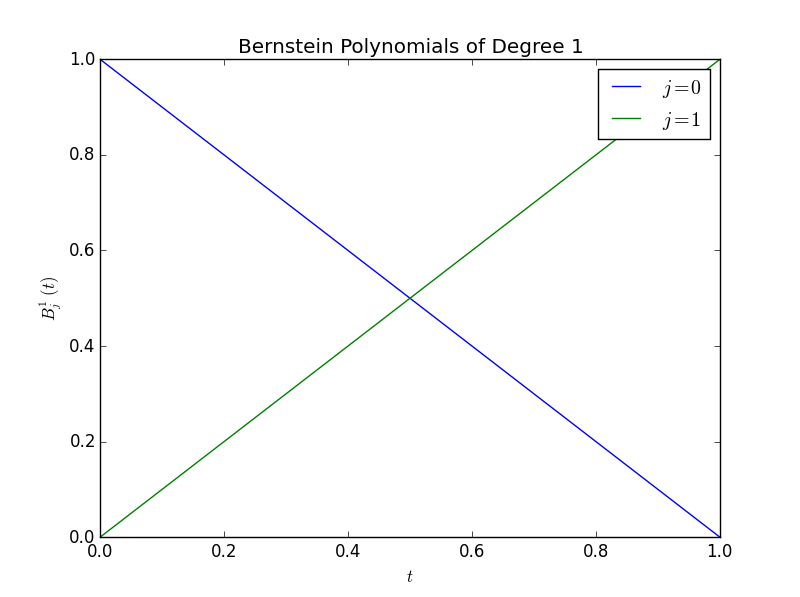
\includegraphics[scale=0.4]{Bernstein_deg1}
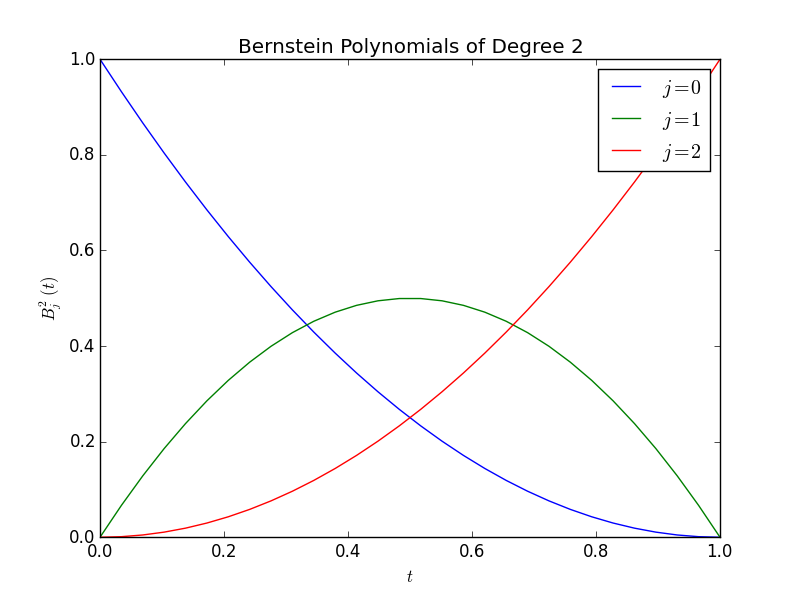
\includegraphics[scale=0.4]{Bernstein_deg2}
\hspace*{-2cm}
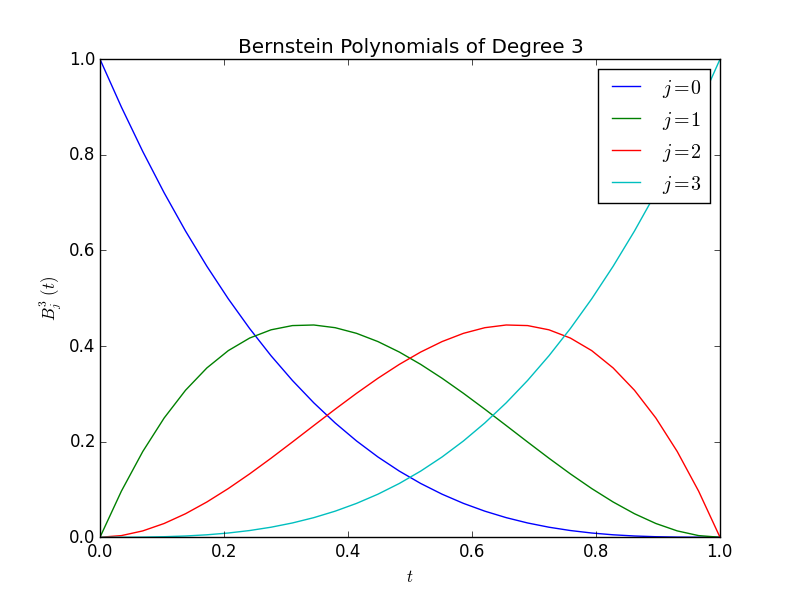
\includegraphics[scale=0.4]{Bernstein_deg3}
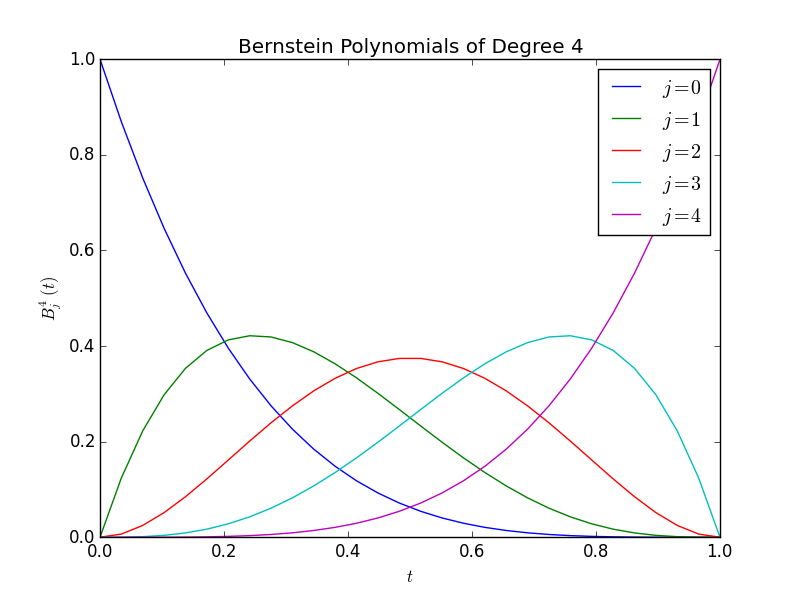
\includegraphics[scale=0.4]{Bernstein_deg4}
\end{figure}

\end{document}
